\chapter{Standard Library Data Structures}
\label{chap:standard_ds}

The purpose of this chapter is to provide an overview on how the most basic and useful data structures work. The implementations of most higher-level languages already coded these for us, but it is important to know how each data structure works rather than blindly use the standard library.

More technical explanations of all of these can be found in a language's API. For Java, this is mostly under the package \texttt{java.util}, in the \href{https://docs.oracle.com/javase/8/docs/api/}{Java API}.

I strongly believe that Java is better than C++ for beginning programmers. It forces people into good coding habits, and though the lack of pointers initially frustrated me, it really does make learning general concepts liked LinkedLists much easier, as the intricacies of the C++ pointer no longer distract from the larger idea.

\section{Generics}
\label{sec:generics}

In general, a data structure can store any kind of data, ranging from integers to strings to other data structures. We therefore want to implement data structures that can hold any and all kinds of information. When we use a data structure, however, we might want our structure to store only one kind of information: only strings, for example, or only integers. We use \textit{generics} to specify to an external structure that we only want it to store a particular kind of information.

\begin{mylstlisting}
ArrayList<Integer> al = new ArrayList<Integer>();
\end{mylstlisting}

This means that \texttt{al} is an ArrayList of Integers. We can only add Integers into the ArrayList, and anything removed from the ArrayList is guaranteed to be an Integer. We can write \texttt{Integer i = al.get(0)} without any need to cast to an Integer.

I don't think the beginning programmer needs to know how to necessarily code a class that supports generics, since each language has its own complex set of rules governing generics. However, we use the standard library extensively in any coding environment, so it is necessary to use a class that does support generics. I think standard classes are relatively straightforward to use but can be annoying to actually implement.

When examining Java API or explanations of implemented functions in this chapter, the characters \texttt{E}, \texttt{V}, and \texttt{K} all can represent generics. For C++, generics are denoted by strings like \texttt{value\_type}. For example, in Java, when we set \texttt{al = new ArrayList<Integer>()}, \texttt{E} represents \texttt{Integer}. Otherwise, \texttt{E} simply means any object.

\section{List}

A list is a collection of objects with an ordering. The objects are ordered in the sense that each element is associated with an index that represents its placement in the list. Users of a list have control over where in the list each object is and can access a specific element by its index, like in an array.

\subsection{Dynamic Array}

What is nice about an array? We can access or change any element we want in the array in $O(1)$ time. The problem is that an array has fixed length. It's not easy to append an element to the end of an array.

The fix to this is pretty simple. Why not just make a bigger array, and copy everything over to the new array? Then there's more room at the end to add a new element. If the backbone array runs out of space, we create a new array with double the size and keep going as if nothing happened. Therefore we now have an array of extendable size -- a \textit{dynamic array}.

\begin{center}
{
\begin{tikzpicture}[
  thick,
  myrect/.style={
    draw,
    fill=myseagreen,
    rectangle split,
    rectangle split horizontal,
    rectangle split parts=#1,
    rectangle split part align=left,
    text width=5ex,
    text centered
    },
  mycallout/.style={
    shape=rectangle callout,
    rounded corners,
    fill=mysalmon,
    callout absolute pointer={#1},
    callout pointer width=1cm
  }  
]

\node[myrect=3]
  (array1)
  {
  					\strut \texttt{"a"}
  \nodepart{two}	\strut \texttt{"b"}
  \nodepart{three}	\strut \texttt{null}
  };
\foreach \Valor [count=\Valori from 0] in {one ,two ,three }
  \node[below] at (array1.\Valor south) {\Valori};

\node[myrect=3]
  (array2)[below=of array1]
  {
  					\strut \texttt{"a"}
  \nodepart{two}	\strut \texttt{"b"}
  \nodepart{three}	\strut \texttt{"c"}
  };
\foreach \Valor [count=\Valori from 0] in {one ,two ,three }
  \node[below] at (array2.\Valor south) {\Valori};

\node[myrect=6]
  (array3)[below=of array2]
  {
  					\strut \texttt{"a"}
  \nodepart{two}	\strut \texttt{"b"}
  \nodepart{three}	\strut \texttt{"c"}
  \nodepart{four}	\strut \texttt{null}
  \nodepart{five}	\strut \texttt{null}
  \nodepart{six}	\strut \texttt{null}
  };
\foreach \Valor [count=\Valori from 0] in {one ,two ,three , four , five , six }
  \node[below] at (array3.\Valor south) {\Valori};

\node[myrect=6]
  (array4)[below=of array3]
  {
  					\strut \texttt{"a"}
  \nodepart{two}	\strut \texttt{"b"}
  \nodepart{three}	\strut \texttt{"c"}
  \nodepart{four}	\strut \texttt{"d"}
  \nodepart{five}	\strut \texttt{null}
  \nodepart{six}	\strut \texttt{null}
  };
\foreach \Valor [count=\Valori from 0] in {one ,two ,three , four , five , six }
  \node[below] at (array4.\Valor south) {\Valori};

\end{tikzpicture}
}
\end{center}

We see that there is still room in the array to add \texttt{"c"}, but to add more elements to the list, we must use a new array with double the length.

It's important to note that any given insertion to the structure is either $O(n)$ or $O(1)$, but there is only one $O(n)$ insertion for every $O(n)$ $O(1)$ insertions, so we still average out to constant time.

The Java implementation of a dynamic array is the \texttt{ArrayList}. The C++ implementation is the \texttt{vector}.

For the following operations, think about how you would implement each and analyze its time complexity. 

\begin{center}
    \begin{tabular}{ p{5cm} p{5cm} p{5cm} }
	Function	&	Java, \texttt{ArrayList}	&	C++, \texttt{vector} \\
	\hline
	\textit{add} an element to the end of the list		&	\texttt{boolean add(E e)}	&	\texttt{void push\_back(const value\_type\& val)}\footnote{\texttt{\& is a C++ reference}} \\
	\textit{insert} an element to a particular index in the list, shifting all subsequent elements down one index	&	\texttt{void add(int index, E element)}		&	\texttt{iterator insert(iterator position, const value\_type\& val)}\footnote{An \textit{iterator} is like a pointer that allows for traversal of a data structure in a particular order. For example, we can increment the iterator to access the next element in the list. An iterator is NOT merely an integer representing the relative position in our list, as the in the Java implementation of \texttt{add}}	\\
	\textit{access} the element stored at a particular index	&	\texttt{E get(int index)}		&	\texttt{reference operator[] (size\_type n)}\footnote{\texttt{size\_type} is, for our purposes, \texttt{unsigned int}, and \texttt{reference operator[]} makes this structure's syntax more like a normal array. In particular, to access the element at index \texttt{i} of a vector \texttt{v}, we simply use \texttt{v[i]}, and to update an element, we use \texttt{v[i] = val}.}	\\
	\textit{update} the value of the element stored at a particular index to a new element & \texttt{E set(int index, E element)} & \texttt{reference operator[] (size\_type n)} \\
	\textit{search} whether the list contains a particular element & \texttt{boolean contains(Object o)} & \texttt{template <class InputIterator, class T>
   InputIterator find (InputIterator first, InputIterator last, const T\& val)}\footnote{This function is in \texttt{<algorithm>}.} \\
	\textit{remove} the element at a particular index from the list & \texttt{E remove(int index)} & \texttt{iterator erase (iterator position)} \\
	search for and \textit{remove} a given element from the list & \texttt{boolean remove(Object o)} & use iterators \\
	return the \textit{size} of the list\footnote{Note that the length of the list is not simply the size of the backing array.} & \texttt{int size()} & \texttt{size\_type size() const}
    \end{tabular}
\end{center}

Accessing and updating elements at particular indices are very nice. They are easy to code and run in constant time. These are the bread and butter of any array. Adding at the end of the list is nice as well. Checking whether some element is contained in the list is a pain, as it is $O(n)$, and adding to and removing from early in the list are more annoying.

\subsection{Linked List}

Arrays are nice for accessing, say, the seventh element in the list. We extend this to the dynamic array to implement adding and removing elements to and from the end of the list nicely. Removing elements from the beginning of the list, however, is cumbersome.

The \textit{linked list} attempts to remedy this. It trades $O(1)$ access to any element in the list for an easier way to remove elements from either end of the list easily. Consider a chain of paper clips:

\begin{center}

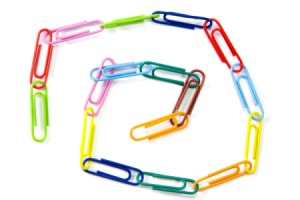
\includegraphics{images/paper_clip_chain.jpg}\footnote{\url{http://img.thrfun.com/img/078/156/paper_clip_chain_s1.jpg}}

\end{center}

It's easy to add or remove more paper clips from either end of the chain, and from any given paper clip, it's easy to access the paper clip directly previous or next to it in the chain. If we needed the seventh paper clip in the chain, we'd need to manually count, an $O(n)$ operation. However, if we then needed to remove that paper clip from the chain, it wouldn't be that hard, assuming we kept a finger, or pointer, on the seventh paper clip.

The best way to think about and implement a linked list is through a cyclical doubly-linked list, with a dummy head. This means each element has its own node container, while the head of the list is simply a node without an element. Such a data structure looks something like this:

\begin{center}


\begin{tikzpicture}[
        list/.style={
            very thick, rectangle split, 
            rectangle split parts=3, draw, 
            rectangle split horizontal, minimum size=18pt,
            inner sep=5pt, text=black,
            rectangle split part fill=myseagreen
        }, 
        ->, start chain, very thick
      ]

  \node[list,on chain] (dummy) {\nodepart{second} \texttt{null}};
  \node[list,on chain] (A) {\nodepart{second} \texttt{"a"}};
  \node[list,on chain] (B) {\nodepart{second} \texttt{"b"}};
  \node[list,on chain] (C) {\nodepart{second} \texttt{"c"}};

    \path[*->] let \p1 = (dummy.three), \p2 = (dummy.center) in (\x1,\y2) edge [bend left] ($(A.one)+(0,0.2)$);
  \path[*->] let \p1 = (A.three), \p2 = (A.center) in (\x1,\y2) edge [bend left] ($(B.one)+(0,0.2)$);
  \path[*->] let \p1 = (B.three), \p2 = (B.center) in (\x1,\y2) edge [bend left] ($(C.one)+(0,0.2)$);
  
%  \draw[*->] let \p1 = (C.three), \p2 = (C.center) in (\x1,\y2) -- (dummy);

%  \draw[*->] ($(A.one)+(0.2,0.1)$) -- (dummy);
  \path[*->] ($(B.one)+(0.1,0.1)$) edge [bend left] ($(A.three)+(0,-0.05)$);
  \path[*->] ($(C.one)+(0.1,0.1)$) edge [bend left] ($(B.three)+(0,-0.05)$);
    \path[*->] ($(A.one)+(0.1,0.1)$) edge [bend left] ($(dummy.three)+(0,-0.05)$);
    
    \draw[*->] ($(C.three)+(0.0,0.2)$) -- ($(C.three)+(1.0,0.2)$) -- ($(C.three)+(1.0,-0.8)$) -- ($(dummy.one)+(-0.9,-0.8)$) -- ($(dummy.one)+(-0.9,0.2)$) -- ($(dummy.one)+(0.1,0.2)$);

    \draw[<-*] ($(C.three)+(0.0,0.0)$) -- ($(C.three)+(0.8,0.0)$) -- ($(C.three)+(0.8,-0.6)$) -- ($(dummy.one)+(-0.7,-0.6)$) -- ($(dummy.one)+(-0.7,0.0)$) -- ($(dummy.one)+(0.1,0.0)$);

\end{tikzpicture}

\end{center}

We see that each node maintains a pointer to its next neighbor and its previous neighbor, in addition to containing the String it stores. We can store this data in a class like the following:

\begin{mylstlisting}
class ListNode<E> {
	ListNode prev, next;
    E s;
}
\end{mylstlisting}

If we were to insert an element after a ListNode \texttt{a}, it is necessary to update all pointers:

\begin{mylstlisting}
ListNode<String> b = new ListNode<String>();
b.prev = a;
b.next = a.next;
b.next.prev = b;
a.next = b;
\end{mylstlisting}

Since the linked list is symmetric, inserting an element before a node is also easy. To add something to the end of the list, simply add it before the dummy head. From here it should not be too hard to implement all the important functions of a linked list.

The Java implementation of a linked list is \texttt{LinkedList}, and the C++ implementation is \texttt{list}. A second C++ class that performs the same tasks but uses a backing array instead of a linked list structure is the \texttt{deque}.

\begin{center}
    \begin{tabular}{ p{3cm} p{4cm} p{4cm} p{4cm} }
	Function	&	Java, \texttt{LinkedList}	&	C++, \texttt{list} & C++, \texttt{deque} \\
	\hline
\textit{add} an element to the end & \texttt{boolean add(E e)} & \multicolumn{2}{p{8cm}}{\centering \texttt{void push\_back(const value\_type\& val)}} \\
\textit{insert}\footnote{The index in a linked list is implicit.} & \texttt{void add(int index, E element)} & \multicolumn{2}{p{8cm}}{\centering \texttt{iterator insert(iterator position, const value\_type\& val)}} \\
\textit{access} & \texttt{E get(int index)} & use iterators & \texttt{reference operator[] (size\_type n)} \\
\textit{update} & \texttt{E set(int index, E element)} & use iterators & \texttt{reference operator[] (size\_type n)} \\
\textit{search} & \texttt{boolean contains(Object o)} & \multicolumn{2}{p{8cm}}{\centering InputIterator find (InputIterator first, InputIterator last, const T\& val)}\footnote{This function is in \texttt{<algorithm>}.} \\
\textit{remove} the element at a particular index & \texttt{E remove(int index)} & \multicolumn{2}{p{8cm}}{\centering \texttt{iterator erase (iterator position)}} \\
search for and \textit{remove} a given element & \texttt{boolean remove(Object o)} & \texttt{void remove (const value\_type\& val)} & use iterators \\
\textit{size} & \texttt{int size()} & \multicolumn{2}{p{8cm}}{\centering \texttt{size\_type size() const}} \\
end operations & \texttt{addFirst}, \texttt{addLast}, \texttt{getFirst}, \texttt{getLast}, \texttt{removeFirst}, \texttt{removeLast} & \texttt{push\_front}, \texttt{push\_back}, \texttt{pop\_front}, \texttt{pop\_back}
    \end{tabular}
\end{center}

With a linked list implemented, two other data structures immediately follow.

\section{Stack}

A \textit{stack} gets its name from being exactly that: a stack. If we have a stack of papers, we can push things on the top and pop things off the top. Sometimes we peek at to access the element on top but don't actually remove anything. We never do anything with what's on the bottom. This is called \textit{LIFO}: Last In, First Out.

Java implements the stack with \texttt{Stack}, C++ with \texttt{stack}.

\begin{center}
    \begin{tabular}{ p{5cm} p{5cm} p{5cm} }
	Function	&	Java, \texttt{Stack}	&	C++, \texttt{stack} \\
	\hline
	\textit{push}		&	\texttt{E push(E item)}	&	\texttt{void push (const value\_type\& val)} \\
    \textit{pop}			&	\texttt{E poll()}		&	\texttt{void pop()}	\\
	\textit{top}		&	\texttt{E peek()}		&	\texttt{value\_type\& top()}	\\
    \textit{size} & \texttt{int size()} & \texttt{size\_type size() const}
    \end{tabular}
\end{center}

Java implements \texttt{Stack} using an array-like structure. This works just as well, and is faster in practice, but I prefer the linked-list structure as a mathematical concept as it is more elegant in its relationship with the queue and more easily customizable.

\section{Queue}

A \textit{queue} is like a queue waiting in line for lunch. We push to the end and pop from the front. Sometimes we peek at the front but don't actually remove anything. The first person in line gets served first. This is called \textit{FIFO}: First In, First Out.

In Java, \texttt{Queue} is an interface, and in C++, the implementation of the queue is \texttt{queue}.

\begin{center}
    \begin{tabular}{ p{5cm} p{5cm} p{5cm} }
	Function	&	Java, \texttt{Queue}	&	C++, \texttt{queue} \\
	\hline
	\textit{push}		&	\texttt{boolean offer(E e)}	&	\texttt{void push (const value\_type\& val)} \\
    \textit{pop}			&	\texttt{E poll()}		&	\texttt{void pop()}	\\
    \textit{top}		&	\texttt{E peek()}		&	\texttt{value\_type\& front()}	\\
    \textit{size} & \texttt{int size()} & \texttt{size\_type size() const}
    \end{tabular}
\end{center}

Since \texttt{Queue} is an interface in Java, we cannot instantiate a \texttt{Queue}, so the following statement is illegal.

\begin{mylstlisting}
Queue<String> q = new Queue<String>();
\end{mylstlisting}

Instead, we must use \texttt{LinkedList}, so we do something like this:

\begin{mylstlisting}
Queue<String> q = new LinkedList<String>();
\end{mylstlisting}

This is legal because \texttt{LinkedList} implements \texttt{Queue}, making it the standard implementation of the FIFO queue.

\section{Heap}

Quite often a FIFO queue is not always desirable. For example, perhaps the string I want to remove at every given point is the one that is lexicographically least.

A min heap is a tree such that every node is smaller than or equal to all of its children. A max heap is a tree such that every node is larger than or equal to all of its children. Pictured is a complete binary min heap, which will be of use to us.

\begin{center}
\begin{tikzpicture}[very thick,level/.style={sibling distance=70mm/#1}]
\node [vertex] (r){\texttt{"a"}}
  child {
    node [vertex] (a) {\texttt{"b"}}
    child {
      node [vertex] {\texttt{"c"}}
      child {
        node [vertex] {\texttt{"e"}}
        child {node [vertex] {\texttt{"f"}}}
      } 
      child {
        node [vertex] {\texttt{"m"}}
      }
    }
    child {
      node [vertex] {\texttt{"n"}}
      child {node [vertex] {\texttt{"p"}}}
      child {node [vertex] {\texttt{"o"}}}
    }
  }
  child {
    node [vertex] {\texttt{"d"}}
    child {
      node [vertex] {\texttt{"g"}}
      child {node [vertex] {\texttt{"i"}}}
      child {node [vertex] {\texttt{"l"}}}
    }
    child {
      node [vertex] {\texttt{"h"}}
      child {node [vertex] {\texttt{"k"}}}
      child {node [vertex] {\texttt{"j"}}}
    }
  };
\end{tikzpicture}
\end{center}

We see that the root of the tree will always be the smallest element. It is tempting to use a container class with a pointer to its left and its right child. However, we have a much nicer way to store \textit{complete} binary trees with an array. Consider the following numbering of the nodes:

\begin{center}
\begin{tikzpicture}[very thick,level 1/.style={sibling distance=80mm}, level 2/.style={sibling distance=40mm}, level 3/.style={sibling distance=20mm}]
\node [splitvertex] (r){1\nodepart{lower}\texttt{"a"}}
  child {
    node [splitvertex] (a) {2\nodepart{lower}\texttt{"b"}}
    child {
      node [splitvertex] {4\nodepart{lower}\texttt{"c"}}
      child {
        node [splitvertex] {8\nodepart{lower}\texttt{"e"}}
        child {node [splitvertex] {16\nodepart{lower}\texttt{"f"}}}
      } 
      child {
        node [splitvertex] {9\nodepart{lower}\texttt{"m"}}
      }
    }
    child {
      node [splitvertex] {5\nodepart{lower}\texttt{"n"}}
      child {node [splitvertex] {10\nodepart{lower}\texttt{"p"}}}
      child {node [splitvertex] {11\nodepart{lower}\texttt{"o"}}}
    }
  }
  child {
    node [splitvertex] {3\nodepart{lower}\texttt{"d"}}
    child {
      node [splitvertex] {6\nodepart{lower}\texttt{"g"}}
      child {node [splitvertex] {12\nodepart{lower}\texttt{"i"}}}
      child {node [splitvertex] {13\nodepart{lower}\texttt{"l"}}}
    }
    child {
      node [splitvertex] {7\nodepart{lower}\texttt{"h"}}
      child {node [splitvertex] {14\nodepart{lower}\texttt{"k"}}}
      child {node [splitvertex] {15\nodepart{lower}\texttt{"j"}}}
    }
  };
\end{tikzpicture}
\end{center}

We see that every number from 1 to 16 is used, and for every node, if the index associated with it is $i$, the left child is $2i$, and the right child is $2i+1$. This leads to a very natural implementation of the tree in an array:

\begin{center}
{
\begin{tikzpicture}[
  thick,
  myrect/.style={
    draw,
    fill=myseagreen,
    rectangle split,
    rectangle split horizontal,
    rectangle split parts=#1,
    rectangle split part align=left,
    text centered
    },
  mycallout/.style={
    shape=rectangle callout,
    rounded corners,
    fill=mysalmon,
    callout absolute pointer={#1},
    callout pointer width=1cm
  }  
]

\node[myrect=17]
  (array)
  {
  					\strut \texttt{null}
  \nodepart{two}	\strut \texttt{"a"}
  \nodepart{three}	\strut \texttt{"b"}
  \nodepart{four}	\strut \texttt{"d"}
  \nodepart{five}	\strut \texttt{"c"}
  \nodepart{six}	\strut \texttt{"n"}
  \nodepart{seven}	\strut \texttt{"g"}
  \nodepart{eight}	\strut \texttt{"h"}
  \nodepart{nine}	\strut \texttt{"e"}
  \nodepart{ten}	\strut \texttt{"m"}
  \nodepart{eleven}	\strut \texttt{"p"}
  \nodepart{twelve}	\strut \texttt{"o"}
  \nodepart{thirteen}	\strut \texttt{"i"}
  \nodepart{fourteen}	\strut \texttt{"l"}
  \nodepart{fifteen}	\strut \texttt{"k"}
  \nodepart{sixteen}	\strut \texttt{"j"}
  \nodepart{seventeen}	\strut \texttt{"f"}
  };
\foreach \Valor [count=\Valori from 0] in {one ,two ,three ,four ,five ,six ,seven ,eight ,nine ,ten ,eleven ,twelve ,thirteen ,fourteen ,fifteen ,sixteen ,seventeen }
  \node[below] at (array.\Valor south) {\Valori};

\end{tikzpicture}
}
\end{center}

How do we add elements to our heap, while maintaining the heap qualities? Well, let's just add it to the very end and see what we get. Suppose we are to add \texttt{"b"} to the tree.

\begin{center}
\begin{tikzpicture}[very thick,level 1/.style={sibling distance=80mm}, level 2/.style={sibling distance=40mm}, level 3/.style={sibling distance=20mm}]
\node [splitvertex] (r){1\nodepart{lower}\texttt{"a"}}
  child {
    node [splitvertex] (a) {2\nodepart{lower}\texttt{"b"}}
    child {
      node [splitvertex] {4\nodepart{lower}\texttt{"c"}}
      child {
        node [splitvertex] {8\nodepart{lower}\texttt{"e"}}
        child {node [splitvertex] {16\nodepart{lower}\texttt{"f"}}}
        child {node [splitvertex, fill=mysalmon] {17\nodepart{lower}\texttt{"b"}}}
      } 
      child {
        node [splitvertex] {9\nodepart{lower}\texttt{"m"}}
      }
    }
    child {
      node [splitvertex] {5\nodepart{lower}\texttt{"n"}}
      child {node [splitvertex] {10\nodepart{lower}\texttt{"p"}}}
      child {node [splitvertex] {11\nodepart{lower}\texttt{"o"}}}
    }
  }
  child {
    node [splitvertex] {3\nodepart{lower}\texttt{"d"}}
    child {
      node [splitvertex] {6\nodepart{lower}\texttt{"g"}}
      child {node [splitvertex] {12\nodepart{lower}\texttt{"i"}}}
      child {node [splitvertex] {13\nodepart{lower}\texttt{"l"}}}
    }
    child {
      node [splitvertex] {7\nodepart{lower}\texttt{"h"}}
      child {node [splitvertex] {14\nodepart{lower}\texttt{"k"}}}
      child {node [splitvertex] {15\nodepart{lower}\texttt{"j"}}}
    }
  };
\end{tikzpicture}
\end{center}

Well, \texttt{"b"} comes before \texttt{"e"} in the alphabet, so let's swap the nodes. We are guaranteed that \texttt{"b"} should come before the other child (in this case, \texttt{"f"}) by the transitive property.

\begin{center}
\begin{tikzpicture}[very thick,level 1/.style={sibling distance=80mm}, level 2/.style={sibling distance=40mm}, level 3/.style={sibling distance=20mm}]
\node [splitvertex] (r){1\nodepart{lower}\texttt{"a"}}
  child {
    node [splitvertex] (a) {2\nodepart{lower}\texttt{"b"}}
    child {
      node [splitvertex] {4\nodepart{lower}\texttt{"c"}}
      child {
        node [splitvertex, fill=mysalmon] {8\nodepart{lower}\texttt{"b"}}
        child {node [splitvertex] {16\nodepart{lower}\texttt{"f"}}}
        child {node [splitvertex, fill=mysalmon] {17\nodepart{lower}\texttt{"e"}}}
      } 
      child {
        node [splitvertex] {9\nodepart{lower}\texttt{"m"}}
      }
    }
    child {
      node [splitvertex] {5\nodepart{lower}\texttt{"n"}}
      child {node [splitvertex] {10\nodepart{lower}\texttt{"p"}}}
      child {node [splitvertex] {11\nodepart{lower}\texttt{"o"}}}
    }
  }
  child {
    node [splitvertex] {3\nodepart{lower}\texttt{"d"}}
    child {
      node [splitvertex] {6\nodepart{lower}\texttt{"g"}}
      child {node [splitvertex] {12\nodepart{lower}\texttt{"i"}}}
      child {node [splitvertex] {13\nodepart{lower}\texttt{"l"}}}
    }
    child {
      node [splitvertex] {7\nodepart{lower}\texttt{"h"}}
      child {node [splitvertex] {14\nodepart{lower}\texttt{"k"}}}
      child {node [splitvertex] {15\nodepart{lower}\texttt{"j"}}}
    }
  };
\end{tikzpicture}
\end{center}

One more swap...

\begin{center}
\begin{tikzpicture}[very thick,level 1/.style={sibling distance=80mm}, level 2/.style={sibling distance=40mm}, level 3/.style={sibling distance=20mm}]
\node [splitvertex] (r){1\nodepart{lower}\texttt{"a"}}
  child {
    node [splitvertex] (a) {2\nodepart{lower}\texttt{"b"}}
    child {
      node [splitvertex, fill=mysalmon] {4\nodepart{lower}\texttt{"b"}}
      child {
        node [splitvertex, fill=mysalmon] {8\nodepart{lower}\texttt{"c"}}
        child {node [splitvertex] {16\nodepart{lower}\texttt{"f"}}}
        child {node [splitvertex] {17\nodepart{lower}\texttt{"e"}}}
      } 
      child {
        node [splitvertex] {9\nodepart{lower}\texttt{"m"}}
      }
    }
    child {
      node [splitvertex] {5\nodepart{lower}\texttt{"n"}}
      child {node [splitvertex] {10\nodepart{lower}\texttt{"p"}}}
      child {node [splitvertex] {11\nodepart{lower}\texttt{"o"}}}
    }
  }
  child {
    node [splitvertex] {3\nodepart{lower}\texttt{"d"}}
    child {
      node [splitvertex] {6\nodepart{lower}\texttt{"g"}}
      child {node [splitvertex] {12\nodepart{lower}\texttt{"i"}}}
      child {node [splitvertex] {13\nodepart{lower}\texttt{"l"}}}
    }
    child {
      node [splitvertex] {7\nodepart{lower}\texttt{"h"}}
      child {node [splitvertex] {14\nodepart{lower}\texttt{"k"}}}
      child {node [splitvertex] {15\nodepart{lower}\texttt{"j"}}}
    }
  };
\end{tikzpicture}
\end{center}

And now we have the heap property restored. As the tree has depth at most $\log{n}$, this process is $O(\log{n})$.

To remove the root from the heap, we replace the root with the last leaf:

\begin{center}
\begin{tikzpicture}[very thick,level 1/.style={sibling distance=80mm}, level 2/.style={sibling distance=40mm}, level 3/.style={sibling distance=20mm}]
\node [splitvertex, fill=mysalmon] (r){1\nodepart{lower}\texttt{"e"}}
  child {
    node [splitvertex] (a) {2\nodepart{lower}\texttt{"b"}}
    child {
      node [splitvertex] {4\nodepart{lower}\texttt{"b"}}
      child {
        node [splitvertex] {8\nodepart{lower}\texttt{"c"}}
        child {node [splitvertex] {16\nodepart{lower}\texttt{"f"}}}
      } 
      child {
        node [splitvertex] {9\nodepart{lower}\texttt{"m"}}
      }
    }
    child {
      node [splitvertex] {5\nodepart{lower}\texttt{"n"}}
      child {node [splitvertex] {10\nodepart{lower}\texttt{"p"}}}
      child {node [splitvertex] {11\nodepart{lower}\texttt{"o"}}}
    }
  }
  child {
    node [splitvertex] {3\nodepart{lower}\texttt{"d"}}
    child {
      node [splitvertex] {6\nodepart{lower}\texttt{"g"}}
      child {node [splitvertex] {12\nodepart{lower}\texttt{"i"}}}
      child {node [splitvertex] {13\nodepart{lower}\texttt{"l"}}}
    }
    child {
      node [splitvertex] {7\nodepart{lower}\texttt{"h"}}
      child {node [splitvertex] {14\nodepart{lower}\texttt{"k"}}}
      child {node [splitvertex] {15\nodepart{lower}\texttt{"j"}}}
    }
  };
  \node [splitvertex, fill=mysalmon] [right=5cm of r]{17\nodepart{lower}\texttt{"a"}};
\end{tikzpicture}
\end{center}

We perform a series of swaps to restore the heap property. We always want to choose the smaller child to swap until the heap property is satisfied.

\begin{center}
\begin{tikzpicture}[very thick,level 1/.style={sibling distance=80mm}, level 2/.style={sibling distance=40mm}, level 3/.style={sibling distance=20mm}, level distance=12mm, level 4/.style={level distance=15mm}]
\node [splitvertex, fill=mysalmon] (r){1\nodepart{lower}\texttt{"b"}}
  child {
    node [splitvertex, fill=mysalmon] (a) {2\nodepart{lower}\texttt{"e"}}
    child {
      node [splitvertex] {4\nodepart{lower}\texttt{"b"}}
      child {
        node [splitvertex] {8\nodepart{lower}\texttt{"c"}}
        child {node [splitvertex] {16\nodepart{lower}\texttt{"f"}}}
      } 
      child {
        node [splitvertex] {9\nodepart{lower}\texttt{"m"}}
      }
    }
    child {
      node [splitvertex] {5\nodepart{lower}\texttt{"n"}}
      child {node [splitvertex] {10\nodepart{lower}\texttt{"p"}}}
      child {node [splitvertex] {11\nodepart{lower}\texttt{"o"}}}
    }
  }
  child {
    node [splitvertex] {3\nodepart{lower}\texttt{"d"}}
    child {
      node [splitvertex] {6\nodepart{lower}\texttt{"g"}}
      child {node [splitvertex] {12\nodepart{lower}\texttt{"i"}}}
      child {node [splitvertex] {13\nodepart{lower}\texttt{"l"}}}
    }
    child {
      node [splitvertex] {7\nodepart{lower}\texttt{"h"}}
      child {node [splitvertex] {14\nodepart{lower}\texttt{"k"}}}
      child {node [splitvertex] {15\nodepart{lower}\texttt{"j"}}}
    }
  };
  \node [splitvertex] [right=5cm of r]{17\nodepart{lower}\texttt{"a"}};
\end{tikzpicture}
\end{center}

\begin{center}
\begin{tikzpicture}[very thick,level 1/.style={sibling distance=80mm}, level 2/.style={sibling distance=40mm}, level 3/.style={sibling distance=20mm}, level distance=12mm, level 4/.style={level distance=15mm}]
\node [splitvertex] (r){1\nodepart{lower}\texttt{"b"}}
  child {
    node [splitvertex, fill=mysalmon] (a) {2\nodepart{lower}\texttt{"b"}}
    child {
      node [splitvertex, fill=mysalmon] {4\nodepart{lower}\texttt{"e"}}
      child {
        node [splitvertex] {8\nodepart{lower}\texttt{"c"}}
        child {node [splitvertex] {16\nodepart{lower}\texttt{"f"}}}
      } 
      child {
        node [splitvertex] {9\nodepart{lower}\texttt{"m"}}
      }
    }
    child {
      node [splitvertex] {5\nodepart{lower}\texttt{"n"}}
      child {node [splitvertex] {10\nodepart{lower}\texttt{"p"}}}
      child {node [splitvertex] {11\nodepart{lower}\texttt{"o"}}}
    }
  }
  child {
    node [splitvertex] {3\nodepart{lower}\texttt{"d"}}
    child {
      node [splitvertex] {6\nodepart{lower}\texttt{"g"}}
      child {node [splitvertex] {12\nodepart{lower}\texttt{"i"}}}
      child {node [splitvertex] {13\nodepart{lower}\texttt{"l"}}}
    }
    child {
      node [splitvertex] {7\nodepart{lower}\texttt{"h"}}
      child {node [splitvertex] {14\nodepart{lower}\texttt{"k"}}}
      child {node [splitvertex] {15\nodepart{lower}\texttt{"j"}}}
    }
  };
  \node [splitvertex] [right=5cm of r]{17\nodepart{lower}\texttt{"a"}};
\end{tikzpicture}
\end{center}

\begin{center}
\begin{tikzpicture}[very thick,level 1/.style={sibling distance=80mm}, level 2/.style={sibling distance=40mm}, level 3/.style={sibling distance=20mm}, level distance=12mm, level 4/.style={level distance=15mm}]
\node [splitvertex] (r){1\nodepart{lower}\texttt{"b"}}
  child {
    node [splitvertex] (a) {2\nodepart{lower}\texttt{"b"}}
    child {
      node [splitvertex, fill=mysalmon] {4\nodepart{lower}\texttt{"c"}}
      child {
        node [splitvertex, fill=mysalmon] {8\nodepart{lower}\texttt{"e"}}
        child {node [splitvertex] {16\nodepart{lower}\texttt{"f"}}}
      } 
      child {
        node [splitvertex] {9\nodepart{lower}\texttt{"m"}}
      }
    }
    child {
      node [splitvertex] {5\nodepart{lower}\texttt{"n"}}
      child {node [splitvertex] {10\nodepart{lower}\texttt{"p"}}}
      child {node [splitvertex] {11\nodepart{lower}\texttt{"o"}}}
    }
  }
  child {
    node [splitvertex] {3\nodepart{lower}\texttt{"d"}}
    child {
      node [splitvertex] {6\nodepart{lower}\texttt{"g"}}
      child {node [splitvertex] {12\nodepart{lower}\texttt{"i"}}}
      child {node [splitvertex] {13\nodepart{lower}\texttt{"l"}}}
    }
    child {
      node [splitvertex] {7\nodepart{lower}\texttt{"h"}}
      child {node [splitvertex] {14\nodepart{lower}\texttt{"k"}}}
      child {node [splitvertex] {15\nodepart{lower}\texttt{"j"}}}
    }
  };
  \node [splitvertex] [right=5cm of r]{17\nodepart{lower}\texttt{"a"}};
\end{tikzpicture}
\end{center}

And we are done. Once again, this takes at most $\log(N)$ swaps. This idea can be extended to removing or changing the value of any node we'd like from a tree -- this is particularly useful for Dijkstra later.

Remember to implement your heap in an array-like structure!

Java implements a min heap with the \texttt{PriorityQueue}. This class, like \texttt{LinkedList}, also implements \texttt{Queue}. C++ implements a \textit{max}\footnote{Don't forget that C++ implements a max heap, ever.} heap with the \texttt{priority\_queue}. The functions for heaps in both languages are nearly identical to those for queues.

\begin{center}
    \begin{tabular}{ p{5cm} p{5cm} p{5cm} }
	Function	&	Java, \texttt{PriorityQueue}	&	C++, \texttt{priority\_queue} \\
	\hline
	\textit{push}		&	\texttt{boolean offer(E e)}	&	\texttt{void push (const value\_type\& val)} \\
    \textit{pop}			&	\texttt{E poll()}		&	\texttt{void pop()}	\\
    \textit{top}		&	\texttt{E peek()}		&	\texttt{value\_type\& top()}	\\
    \textit{size} & \texttt{int size()} & \texttt{size\_type size() const}
    \end{tabular}
\end{center}

\section{Set}

A \textit{set} is a collection of objects with no duplicate elements. Note that the data structures discussed in this section can be extended to become multisets, but Java and C++ implementations of these explicitly disallow multiplicity.

\subsection{Binary Search Tree}

A \textit{binary search tree (BST)} is a tree where every node is greater than every node in its left subtree and less than every node in its right subtree. As with a heap, to use a BST, we need to impose some kind of ordering on the elements stored.

\begin{center}
\begin{tikzpicture}[very thick,level/.style={sibling distance=70mm/#1}]
\node [vertex] (r){\texttt{"m"}}
  child {
    node [vertex] {\texttt{"g"}}
    child {
      node [vertex] {\texttt{"c"}}
      child {
        node [vertex] {\texttt{"b"}}
        child {node [vertex] {\texttt{"a"}}}
        child[missing]
      } 
      child {
        node [vertex] {\texttt{"e"}}
      }
    }
    child {
      node [vertex] {\texttt{"j"}}
      child {node [vertex] {\texttt{"h"}}}
      child {node [vertex] {\texttt{"k"}}}
    }
  }
  child {
    node [vertex] {\texttt{"t"}}
    child {
      node [vertex] {\texttt{"r"}}
      child[missing]
      child {node [vertex] {\texttt{"s"}}}
    }
    child[missing]
  };
\end{tikzpicture}
\end{center}

The tree need not be complete, unlike the heap. Because it is not guaranteed to be complete, there is no way to nicely bound the size of the array we would need if we were to use the same storage method as with the heap. Thus, we are forced to use a \texttt{TreeNode}, with left and right pointers. This is also problematic when determining guarantees on time complexities later, but the ways to solve this problem are pretty complicated so we'll ignore them for now.

Given the name of the tree, searching for an element within the tree is quite natural, and similar to a binary search. Compare the element to be searched for with the current node. If they are equal, we are done; otherwise, search the appropriate left or right subtree. As with most structures and algorithms with a binary search structure, this operation lends itself nicely to recursion. If the tree is reasonably nice, we expect to complete this in $O(\log{n})$ time, but searching can be as bad as linear if the tree looks like a linked list.

Adding an element is also natural. As our tree represents a set, it will not contain the same element twice. We trace down until we hit a null pointer, and add the element in the appropriate spot. Let's add a \texttt{"p"} to the BST:

\begin{center}
\begin{tikzpicture}[very thick,level/.style={sibling distance=70mm/#1}]
\node [vertex, fill=mysalmon] (r){\texttt{"m"}}
  child {
    node [vertex] {\texttt{"g"}}
    child {
      node [vertex] {\texttt{"c"}}
      child {
        node [vertex] {\texttt{"b"}}
        child {node [vertex] {\texttt{"a"}}}
        child[missing]
      } 
      child {
        node [vertex] {\texttt{"e"}}
      }
    }
    child {
      node [vertex] {\texttt{"j"}}
      child {node [vertex] {\texttt{"h"}}}
      child {node [vertex] {\texttt{"k"}}}
    }
  }
  child {
    node [vertex, fill=mysalmon] {\texttt{"t"}}
    child {
      node [vertex, fill=mysalmon] {\texttt{"r"}}
      child {node [vertex, fill=mysalmon] {\texttt{"p"}}}
      child {node [vertex] {\texttt{"s"}}}
    }
    child[missing]
  };
\end{tikzpicture}
\end{center}

Deleting an element is the annoying part. Unfortunately, there's not much we can do besides casework.

Removing a leaf, like \texttt{"a"}, from the tree is very easy. Removing a node with only once child, like \texttt{"t"}, is also relatively straightforward.

\begin{center}
\begin{tikzpicture}[very thick,level/.style={sibling distance=70mm/#1}]
\node [vertex] (r){\texttt{"m"}}
  child {
    node [vertex] {\texttt{"g"}}
    child {
      node [vertex] {\texttt{"c"}}
      child {
        node [vertex] {\texttt{"b"}}
        child {node [vertex,fill=mysalmon] {\texttt{"a"}}}
        child[missing]
      } 
      child {
        node [vertex] {\texttt{"e"}}
      }
    }
    child {
      node [vertex] {\texttt{"j"}}
      child {node [vertex] {\texttt{"h"}}}
      child {node [vertex] {\texttt{"k"}}}
    }
  }
  child {
    node [vertex, fill=mysalmon] {\texttt{"t"}}
    child {
      node [vertex] {\texttt{"r"}}
      child {node [vertex] {\texttt{"p"}}}
      child {node [vertex] {\texttt{"s"}}}
    }
    child[missing]
  };
\end{tikzpicture}
\end{center}

Now, removing an element with two children is tricky. We'll try to remove \texttt{"g"}. Consider the least element in the right subtree of \texttt{"g"}, which in this case is \texttt{"h"}. We find \texttt{"h"} by always choosing the left child on the right subtree until we cannot go any further. This must be the least element.

\begin{center}
\begin{tikzpicture}[very thick,level/.style={sibling distance=70mm/#1}]
\node [vertex] (r){\texttt{"m"}}
  child {
    node [vertex, fill=mysalmon] {\texttt{"g"}}
    child {
      node [vertex] {\texttt{"c"}}
      child {
        node [vertex] {\texttt{"b"}}
      } 
      child {
        node [vertex] {\texttt{"e"}}
      }
    }
    child {
      node [vertex] {\texttt{"j"}}
      child {node [vertex] {\texttt{"h"}}}
      child {node [vertex] {\texttt{"k"}}}
    }
  }
  child {
      node [vertex] {\texttt{"r"}}
      child {node [vertex] {\texttt{"p"}}}
      child {node [vertex] {\texttt{"s"}}}
  };
\end{tikzpicture}
\end{center}

Note that \texttt{"h"} has either no children or only one child, and that nodes like these are easy to remove. We then change the value of the node containing \texttt{"g"} to \texttt{"h"}, which is legal since \texttt{"h"} is the least element, and remove \texttt{"h"} from the right subtree, and we are done.

\begin{center}
\begin{tikzpicture}[very thick,level/.style={sibling distance=70mm/#1}]
\node [vertex] (r){\texttt{"m"}}
  child {
    node [vertex, fill=mysalmon] {\texttt{"h"}}
    child {
      node [vertex] {\texttt{"c"}}
      child {
        node [vertex] {\texttt{"b"}}
      } 
      child {
        node [vertex] {\texttt{"e"}}
      }
    }
    child {
      node [vertex] {\texttt{"j"}}
      child {node [vertex, fill=mysalmon] {\texttt{"h"}}}
      child {node [vertex] {\texttt{"k"}}}
    }
  }
  child {
      node [vertex] {\texttt{"r"}}
      child {node [vertex] {\texttt{"p"}}}
      child {node [vertex] {\texttt{"s"}}}
  };
\end{tikzpicture}
\end{center}

\begin{center}
\begin{tikzpicture}[very thick,level/.style={sibling distance=70mm/#1}]
\node [vertex] (r){\texttt{"m"}}
  child {
    node [vertex] {\texttt{"h"}}
    child {
      node [vertex] {\texttt{"c"}}
      child {
        node [vertex] {\texttt{"b"}}
      } 
      child {
        node [vertex] {\texttt{"e"}}
      }
    }
      child {node [vertex] {\texttt{"j"}}
      	child[missing]
        child {
        	node[vertex]{\texttt{"k"}}
        }
      }
  }
  child {
      node [vertex] {\texttt{"r"}}
      child {node [vertex] {\texttt{"p"}}}
      child {node [vertex] {\texttt{"s"}}}
  };
\end{tikzpicture}
\end{center}

Since a BST is ordered, iterating over it from left to right will pass over every element in sorted order.

A standard BST has $O(\log{n})$ operations if the tree is ``nice,'' or sufficiently randomized, but each operation can be $O(n)$ in the worst case. We need to find a way to automatically balance the BST such that we avoid linear time complexities.

A red-black tree is a self-balancing BST that guarantees $O(\log{n})$ operations by making sure the height of the tree grows logarithmically. It is implemented in Java's \texttt{TreeSet} and is usually\footnote{Implementations of \texttt{set} must be some kind of balanced binary search tree, but need not be red-black.} implemented in the C++ \texttt{set}, so while the simple BST I described above does not guarantee nice time bounds, Java's implementation does.

I don't think learning exactly how a red-black tree works is particularly useful for the beginning programmer or a competitive programmer. How exactly a red-black tree works, together with some more balanced binary search trees which are useful on the competitive scene, are covered in a later chapter.

\begin{center}
    \begin{tabular}{ p{5cm} p{5cm} p{5cm} }
	Function	&	Java, \texttt{TreeSet}	&	C++, \texttt{set} \\
	\hline
	\textit{insert}		&	\texttt{boolean add(E e)}	&	\texttt{void insert (const value\_type\& val)} \\
   \textit{search}		&	\texttt{boolean contains(Object o)}	&	\texttt{size\_type count (const value\_type\& val) const}\footnote{1 if in the \texttt{set}, 0 otherwise.}	\\
    \textit{delete}		&	\texttt{boolean	remove(Object o)}		&	\texttt{size\_type erase (const value\_type\& val)}, \texttt{void erase (iterator position)} \\
    \textit{size} & \texttt{int size()} & \texttt{size\_type size() const} \\
    other useful \textit{search} functions	& \texttt{first}, \texttt{last}, \texttt{ceiling}, \texttt{floor}, \texttt{higher}, \texttt{lower} & \texttt{begin}, \texttt{end}, \texttt{lower\_bound}\footnote{\texttt{lower\_bound} is similar to Java's \texttt{ceiling}}, \texttt{upper\_bound}\footnote{\texttt{upper\_bound} is similar to Java's \texttt{higher}}
    \end{tabular}
\end{center}

\subsection{Hash Table}

A \textit{hash table} is a way for us to store objects when we do not require a natural ordering on the set. As with the binary search tree, we want to be able to check whether an element is in our set or not quickly. We do this with the help of a \textit{hash function}. The hash function operates on the object and returns something that characterizes that object. For example, for a string, a possible hash could be the length of the string or the sum of the characters. We want to map an object with an integer hash, so that we can store the values by their hashes in an array.

What characterizes a good hash function?

\begin{enumerate}
\item
If two objects are considered equal, like the strings \texttt{"Hello"} and \texttt{"Hello"}, their hashes must be equal.
\item
If two objects are not equal, like the strings \texttt{"Hello"} and \texttt{"Bye"}, their hashes are only equal with very low probability. A \textit{collision} is when two different objects have the same hash. We want to minimize the probability of this happening. As a result, hashes like the length of the string are not very good hashes.
\item
A good hash should be reasonably fast to compute. One main purpose of hashing is to make equality checks between objects fast. A hash function that is hard to compute defeats the purpose of this.
\end{enumerate}

Every Java \texttt{Object} supports the \texttt{hashCode()} function. By default, \texttt{hashCode()} stores information about the memory address of the \texttt{Object}. When we implement a new class, we can override this function. For example, let us define the following \textit{polynomial hash} for strings:

\begin{mylstlisting}
public int hashCode() {
	int hash = 0;
    for(int k = 0; k < length(); k++) {
		hash *= 31;
        hash += (int) (charAt(k));
    }
    return hash;
}
\end{mylstlisting}

In Java, \texttt{a.equals(b)} should imply \texttt{a.hashCode() == b.hashCode()}. This function produces the same result as the actual \texttt{hashCode()} function in the String class. However, this is not quite what we want for our hash set implementation, because in the end we wish to be able to store the objects in some kind of array. Since \texttt{hashCode()} can be any \texttt{int}, this hash not only returns integers that can be very large, they can also be negative, and thus are not suitable as array indices. The natural way to fix this is to take the hash modulo the size of the array we want.

\begin{mylstlisting}
String[] table = new String[10007];
int index(E o) {
	int i = o.hashCode() % table.length;
    if(i >= 0)
    	return i;
	return i + table.length;
}
\end{mylstlisting}

The length of our array is somewhat arbitrary. We chose the number 100007 because it is a prime number, and primes are generally nice since integers modulo a prime form a field. Remember that a negative number \texttt{\%} another number is not necessarily positive, so we need to be a little careful.

From here, adding an element to the table and checking if an element is contained both seem straightforward:

\begin{mylstlisting}
boolean add(E o) {
	table[index(o)] = o;
    return true;
}
boolean contains(Object o) {
    int i = index((E) o);
	return table[i] != null && table[i].equals(o);
}
\end{mylstlisting}

\texttt{null} is always annoying to deal with, and will always have to be handled separately.

However, a problem quickly arises in the (hopefully unlikely) instance of a collision. If two strings have the same hash, we can't add both to the table since there isn't enough space in the array. The easiest way to handle a collision is by \textit{chaining}. We change the hash table to store a linked list instead of a single element in the event of a collision. The hope is that not too many objects map to a single index in the array, as searching a linked list for a particular element is $O(n)$. Java once implemented this method of resolving collisions, but recently changed it to a BST in Java 8.

If we use a good hash function and a reasonable array size, collisions will almost always be pretty evenly spread across the array. Then, since we store everything using an array, the hash table provides probabilistic $O(1)$ time complexities for insertion, deletion, and search.

The Java set implementation of a hash table is the \texttt{HashSet}. The C++11\footnote{added recently; not included in C++} set implementation of a hash table is the \texttt{unordered\_set}.

\begin{center}
    \begin{tabular}{ p{5cm} p{5cm} p{5cm} }
	Function	&	Java, \texttt{HashSet}	&	C++11, \texttt{unordered\_set} \\
	\hline
	\textit{insert}		&	\texttt{boolean add(E e)}	&	\texttt{void insert (const value\_type\& val)} \\
   \textit{search}		&	\texttt{boolean contains(Object o)}	&	\texttt{size\_type count (const value\_type\& val) const}\footnote{1 if in the \texttt{set}, 0 otherwise.}	\\
    \textit{delete}		&	\texttt{boolean	remove(Object o)}		&	\texttt{size\_type erase (const value\_type\& val)}, \texttt{void erase (iterator position)} \\
    \textit{size} & \texttt{int size()} & \texttt{size\_type size() const}
    \end{tabular}
\end{center}

\section{Map}

A map is very similar to a set. A map is simply a function that takes a key to a value. Generics for maps therefore have two arguments: one for the key and one for the value. Consider the following Java \texttt{Map} from \texttt{String}s to \texttt{String}s.

\begin{mylstlisting}
Map<String, String> email = new TreeMap<String, String>();
email.put("Samuel Hsiang", "samuel.c.hsiang@gmail.com");
\end{mylstlisting}

As a map is a function, the domain, or the keys of the map, form a set, though the values need not be unique.

\texttt{Map} is a Java interface. The \texttt{TreeMap} is the \texttt{Map} variant of the \texttt{TreeSet}; similarly, the \texttt{HashMap} is the \texttt{Map} variant of the \texttt{HashSet}. \texttt{map} is the C++ implementation of a balanced binary search tree map, while \texttt{unordered\_map} is the C++11 implementation of a hash table.

\begin{center}
    \begin{tabular}{ p{5cm} p{5cm} p{5cm} }
	Function	&	Java, \texttt{TreeMap}	&	C++, \texttt{map} \\
	\hline
	\textit{insert} and \textit{update}	value	&	\texttt{V put(K key, V value)}	&	\texttt{mapped\_type\& operator[] (const key\_type\& k)}\footnote{Works like an array or \texttt{vector}.} \\
	\textit{access} & \texttt{V get(Object key)} & \texttt{mapped\_type\& operator[] (const key\_type\& k)} \\
    \textit{delete} & \texttt{V remove(Object key)} &	\texttt{size\_type erase (const key\_type\& val)}, \texttt{void erase (iterator position)} \\
    \textit{size} & \texttt{int size()} & \texttt{size\_type size() const} \\
    other useful \textit{search} functions	& \multicolumn{2}{c}{just look in the API >.<}
    \end{tabular}
\end{center}

\begin{center}
    \begin{tabular}{ p{5cm} p{5cm} p{5cm} }
	Function	&	Java, \texttt{HashMap}	&	C++11, \texttt{unordered\_map} \\
	\hline
	\textit{insert} and \textit{update}	value	&	\texttt{V put(K key, V value)}	&	\texttt{mapped\_type\& operator[] (const key\_type\& k)}\footnote{Works like an array or \texttt{vector}.} \\
	\textit{access} & \texttt{V get(Object key)} & \texttt{mapped\_type\& operator[] (const key\_type\& k)} \\
    \textit{delete} & \texttt{V remove(Object key)} &	\texttt{size\_type erase (const key\_type\& val)}, \texttt{void erase (iterator position)} \\
    \textit{size} & \texttt{int size()} & \texttt{size\_type size() const}
    \end{tabular}
\end{center}

\section{Big Integer}

A big int is for times when int and long just aren't large enough. The way it works is it stores a number as an array of ints. Each value in the array represents a digit in some very large base. Addition and subtraction can be done in the standard way. Generally multiplying two big ints is not necessary on contests, but it can be sped up using multiplication algorithms like Karatsuba.

\texttt{BigInteger} is in \texttt{java.math}, but C++ does not have an implementation.
